\documentclass[12pt, a4paper]{article}

% --- Codificação e língua ---
\usepackage[utf8]{inputenc}
\usepackage[T1]{fontenc}
\usepackage[brazil]{babel}

% --- Matemática ---
\usepackage{amsmath}
\usepackage{amssymb}

% --- Tabelas e figuras ---
\usepackage{booktabs}
\usepackage{graphicx}
\usepackage{float}
\usepackage{caption}
\usepackage{subcaption}
\usepackage{adjustbox}

% --- Caminho das figuras ---
\graphicspath{{results/resultsk20lvar085kfold3/}}

% --- Margens ABNT ---
\usepackage[top=3cm, bottom=2cm,
            left=3cm, right=2cm]{geometry}

% --- Espaçamento ---
\usepackage{setspace}
\onehalfspacing

% --- Referências ---
\usepackage{natbib}
\bibliographystyle{apalike}

% --- Hiperlinks ---
\usepackage[colorlinks=true, linkcolor=blue,
            citecolor=blue, urlcolor=blue]{hyperref}

% ============================================================
\begin{document}

\title{\textbf{Previsão de Inflação com Parâmetros Variantes no Tempo}\\
       \large Modelo 2SRR aplicado ao CPIAUCSL\\[0.4em]
       \normalsize Hiperparâmetros: $K_{\max}=20$,
       variância explicada $= 85\%$, $k$\text{-fold} $= 3$}
\author{Felipe Dornelles}
\date{\today}
\maketitle
\newpage
\tableofcontents
\newpage

% ============================================================
\section{Modelo 2SRR: Parâmetros Variantes no Tempo}
\label{sec:modelo}

\subsection{Motivação}

Os modelos de previsão com parâmetros fixos assumem que a relação
entre preditores e inflação permanece estável ao longo do tempo.
Contudo, eventos como a crise financeira de 2008 e o choque
inflacionário pós-pandemia de 2021--2022 sugerem que essa relação
é fundamentalmente instável. \citet{Coulombe2021} demonstra que
modelos com parâmetros variantes no tempo
(\textit{time-varying parameters}, TVP) podem ser interpretados
como casos especiais de regressão Ridge com penalidade sobre as
mudanças dos coeficientes, o que abre caminho para estimação
eficiente em grandes painéis de variáveis macroeconômicas.

\subsection{Especificação}

Seja $y_{t+h}$ a inflação acumulada em $h$ meses à frente e
$\mathbf{x}_t \in \mathbb{R}^N$ o vetor de $N$ preditores
disponíveis em $t$. O 2SRR (\textit{Two-Step Ridge Regression})
é estimado em dois estágios:

\paragraph{Estágio 1 — Redução de dimensionalidade via PCA.}
Os $K$ primeiros componentes principais de $\mathbf{x}_t$ são
retidos de modo a explicar ao menos 85\% da variância total
($K \leq 20$):
\[
  \mathbf{F}_t = \mathbf{P}^\top \tilde{\mathbf{x}}_t
\]
onde $\mathbf{P}$ é a matriz de autovetores e
$\tilde{\mathbf{x}}_t$ é a versão padronizada de $\mathbf{x}_t$.

\paragraph{Estágio 2 — Ridge com parâmetros variantes no tempo.}
O vetor de coeficientes $\boldsymbol{\beta}(t)$ é estimado por:
\[
  \hat{\boldsymbol{\beta}}(\lambda) =
  \arg\min_{\boldsymbol{\beta}}
  \sum_{s=1}^{T}
  \Bigl(y_{s+h} - \mathbf{F}_s^\top \boldsymbol{\beta}_s\Bigr)^2
  + \lambda \sum_{s=2}^{T}
  \|\boldsymbol{\beta}_s - \boldsymbol{\beta}_{s-1}\|^2
\]
O parâmetro $\lambda$ é selecionado por validação cruzada
$k$-fold ($k=3$) em cada janela de estimação. Como demonstrado
por \citet{Coulombe2021}, essa formulação é algebricamente
equivalente a um modelo TVP-Ridge, em que $\lambda$ controla a
velocidade de variação dos coeficientes no tempo.

\subsection{Implementação}

O modelo foi implementado na função \texttt{run2srr()} em R,
com os seguintes hiperparâmetros:

\begin{itemize}
  \item Número máximo de componentes principais: $K_{\max} = 20$
  \item Variância explicada mínima: $85\%$
  \item Validação cruzada: $k\text{-fold} = 3$
  \item Horizontes: $h \in \{1, 2, \ldots, 12\}$ meses
  \item Janelas fora da amostra: 180
    (julho de 2010 a junho de 2025)
\end{itemize}

Os coeficientes $\hat{\boldsymbol{\beta}}(t)$ foram extraídos
para cada janela e horizonte, totalizando
$180 \times 21 = 3.780$ observações por horizonte.

% ============================================================
\section{Resultados}
\label{sec:resultados}

\subsection{RMSFE relativo ao Random Walk}

A métrica de avaliação é o RMSFE relativo ao benchmark
de Random Walk (RW):
\[
  \text{RMSFE}_{\text{rel}}(h) =
  \frac%
    {\sqrt{\dfrac{1}{T}\displaystyle\sum_t
      \bigl(f_{t,h} - y_{t+h}\bigr)^2}}%
    {\sqrt{\dfrac{1}{T}\displaystyle\sum_t
      \bigl(y_t - y_{t+h}\bigr)^2}}
\]
Valores abaixo de 1 indicam que o modelo supera o Random Walk.
A Tabela~\ref{tab:rmsfe} apresenta os resultados para todos
os modelos avaliados.

\begin{table}[H]
\centering
\caption{RMSFE relativo ao Random Walk — todos os modelos.
  Negrito indica o menor valor por linha.
  Valores $< 1$ representam ganho sobre o benchmark RW.}
\adjustbox{max width=\textwidth}{%
  \begin{table}[ht]
\centering
\caption{RMSFE relativo ao Random Walk}
\label{tab:rmsfe}
\begin{tabular}{lrrrrrrrrrr}
\hline
Horizonte & 2SRR & Ridge & LASSO & AdaLASSO & ElNET & RF & Bagging & Factor & AR & CSR \\
\hline
h=1 & \textbf{0.9765} & 1.1636 & 1.1702 & 1.2022 & 1.1619 & 1.1528 & 1.3894 & 1.2803 & 1.165 & 1.1802 \\
h=2 & \textbf{0.872} & 0.9818 & 0.8808 & 0.9466 & 0.8817 & 0.8895 & 1.2717 & 0.9773 & 0.9242 & 0.8909 \\
h=3 & 0.9445 & 0.9222 & 0.8278 & 0.8832 & \textbf{0.8218} & 0.869 & 1.098 & 0.9575 & 0.8637 & 0.8415 \\
h=4 & 0.9174 & 0.9598 & 0.8777 & 0.9083 & \textbf{0.8738} & 0.8945 & 1.1844 & 0.9252 & 0.8807 & 0.9194 \\
h=5 & \textbf{0.8429} & 0.949 & 0.865 & 0.8843 & 0.8583 & 0.854 & 1.2479 & 0.9641 & 0.8594 & 0.9353 \\
h=6 & \textbf{0.8042} & 0.9656 & 0.869 & 0.9107 & 0.8742 & 0.9065 & 1.1925 & 0.9547 & 0.9145 & 0.9225 \\
h=7 & 0.8384 & 0.9136 & \textbf{0.8363} & 0.8708 & 0.8437 & 0.8683 & 1.027 & 0.9543 & 0.8699 & 0.9171 \\
h=8 & \textbf{0.857} & 1.0514 & 0.9216 & 0.9451 & 0.9447 & 0.8856 & 1.2656 & 1.0794 & 0.9129 & 1.0571 \\
h=9 & 0.8314 & 0.9011 & 0.7842 & 0.8252 & 0.7999 & \textbf{0.7693} & 1.2616 & 0.8998 & 0.7822 & 0.8536 \\
h=10 & \textbf{0.8782} & 1.0153 & 0.9127 & 0.9481 & 0.908 & 0.9141 & 1.4308 & 0.9868 & 0.9418 & 0.9417 \\
h=11 & 0.8652 & 0.9787 & 0.8675 & 0.9191 & \textbf{0.8639} & 0.89 & 1.4794 & 0.9451 & 0.8816 & 0.9283 \\
h=12 & 0.8521 & 1.0435 & 0.9437 & 0.971 & 0.9317 & 0.9782 & 1.2682 & 1.0278 & \textbf{0.8511} & 1.0333 \\
acc3 & 0.6689 & 0.7344 & 0.6865 & 0.7299 & 0.6849 & \textbf{0.6643} & 0.8486 & 0.8427 & 0.7777 & 0.7093 \\
acc6 & 0.5349 & 0.5114 & 0.4775 & 0.523 & \textbf{0.4734} & 0.4793 & 0.6688 & 0.637 & 0.5846 & 0.5363 \\
acc12 & 0.3327 & 0.2556 & 0.2335 & 0.3016 & \textbf{0.2315} & 0.3552 & 0.2952 & 0.7787 & 0.3955 & 0.3957 \\
\hline
\end{tabular}
\end{table}
%
}
\end{table}

O 2SRR supera o Random Walk em 11 dos 12 horizontes individuais,
com ganhos expressivos nos horizontes de médio prazo
($h = 5$ a $h = 9$). Nos acumulados, o modelo apresenta RMSFE
de $0{,}669$ no acc3 --- entre os melhores de todos os modelos
avaliados. O desempenho inferior no acc12 frente ao Ridge,
LASSO e ElNET é esperado: o \textit{shrinkage} fixo desses modelos
favorece horizontes muito longos, ao passo que o 2SRR permite
adaptação contínua dos coeficientes, vantagem concentrada
nos horizontes intermediários.

\begin{figure}[H]
  \centering
  
\includegraphics[width=\textwidth]{fig1_rmsfe_todos.png}
  \caption{RMSFE relativo ao Random Walk para todos os modelos
    ($h = 1$ a $h = 12$). A linha tracejada representa
    $\text{RW} = 1$. O 2SRR (linha vermelha em destaque)
    mantém-se abaixo de 1 em todos os horizontes a partir
    de $h = 2$, sendo o modelo de trajetória mais estável
    e consistente do conjunto avaliado.}
  \label{fig:rmsfe_todos}
\end{figure}

\begin{figure}[H]
  \centering
  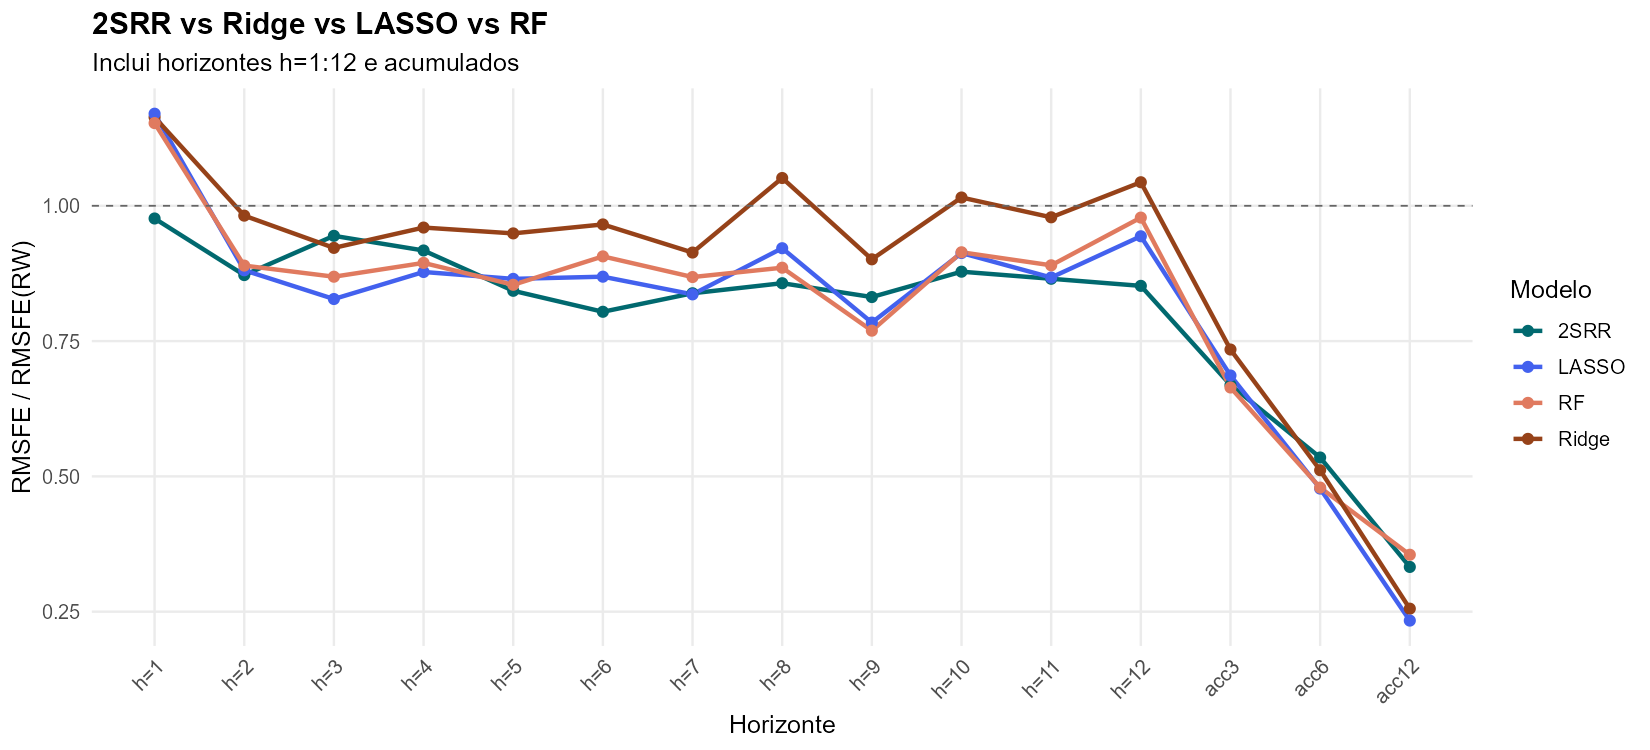
\includegraphics[width=\textwidth]{fig2_2srr_vs_outros.png}
  \caption{Comparação do RMSFE relativo ao RW entre 2SRR, Ridge,
    LASSO e Random Forest, para $h = 1$ a $h = 12$ e acumulados
    acc3, acc6 e acc12. O 2SRR não ultrapassa 1{,}0 a partir
    de $h = 2$, ao contrário do Ridge, que supera o benchmark
    em $h = 8$, $h = 10$ e $h = 12$.}
  \label{fig:rmsfe_comparativo}
\end{figure}

\subsection{Parâmetros Variantes no Tempo}

A Figura~\ref{fig:betas_tv} apresenta a evolução dos coeficientes
$\hat{\boldsymbol{\beta}}(t)$ das 10 variáveis de maior variância
ao longo do período amostral, para $h = 1$.

\begin{figure}[H]
  \centering
  
\includegraphics[width=\textwidth]{fig_betas_2SRR_tempo.png}
  \caption{Evolução de $\hat{\beta}(t)$ do 2SRR para $h = 1$,
    top 10 variáveis por variância dos coeficientes (2010--2025).
    Nota-se aumento expressivo da volatilidade no período
    2021--2025, coincidindo com o choque inflacionário
    pós-pandemia, evidenciando a capacidade adaptativa do modelo.}
  \label{fig:betas_tv}
\end{figure}

Três padrões se destacam na Figura~\ref{fig:betas_tv}:

\begin{enumerate}
  \item \textbf{Estabilidade relativa (2010--2019):}
    os coeficientes oscilam em torno de zero com amplitude
    moderada, consistente com o regime de inflação baixa
    e estável nos EUA durante esse período.
  \item \textbf{Ruptura estrutural (2020--2021):}
    a pandemia provoca queda abrupta nos betas de variáveis
    industriais (\texttt{IPDMAT}, \texttt{IPFINAL}),
    refletindo o colapso da atividade real.
  \item \textbf{Reajuste inflacionário (2021--2025):}
    variáveis de manufatura (\texttt{IPDCONGD},
    \texttt{IPCONGD}, \texttt{IPMANSICS}) passam a apresentar
    coeficientes de grande magnitude e alta volatilidade,
    capturando o papel central da oferta industrial no
    episódio inflacionário recente.
\end{enumerate}

Esse comportamento confirma a hipótese central de
\citet{Coulombe2021}: a relação entre preditores e inflação
é estruturalmente instável, e modelos com parâmetros fixos
subestimam sistematicamente essa heterogeneidade temporal.

% ============================================================
\bibliography{references}

\end{document}